\section{The creature}

We call the system a creature: a small language-model agent that works by day and is fine-tuned at night (its ``sleep'') on lessons chosen by a judge. These names label an ordinary continual fine-tuning loop; they make no claim about biology. Its base model never changes; everything it learns lives in a small LoRA adapter, trained each night on the day's lessons (Fig.~\ref{fig:1}).

\begin{figure}[htbp]
\centering
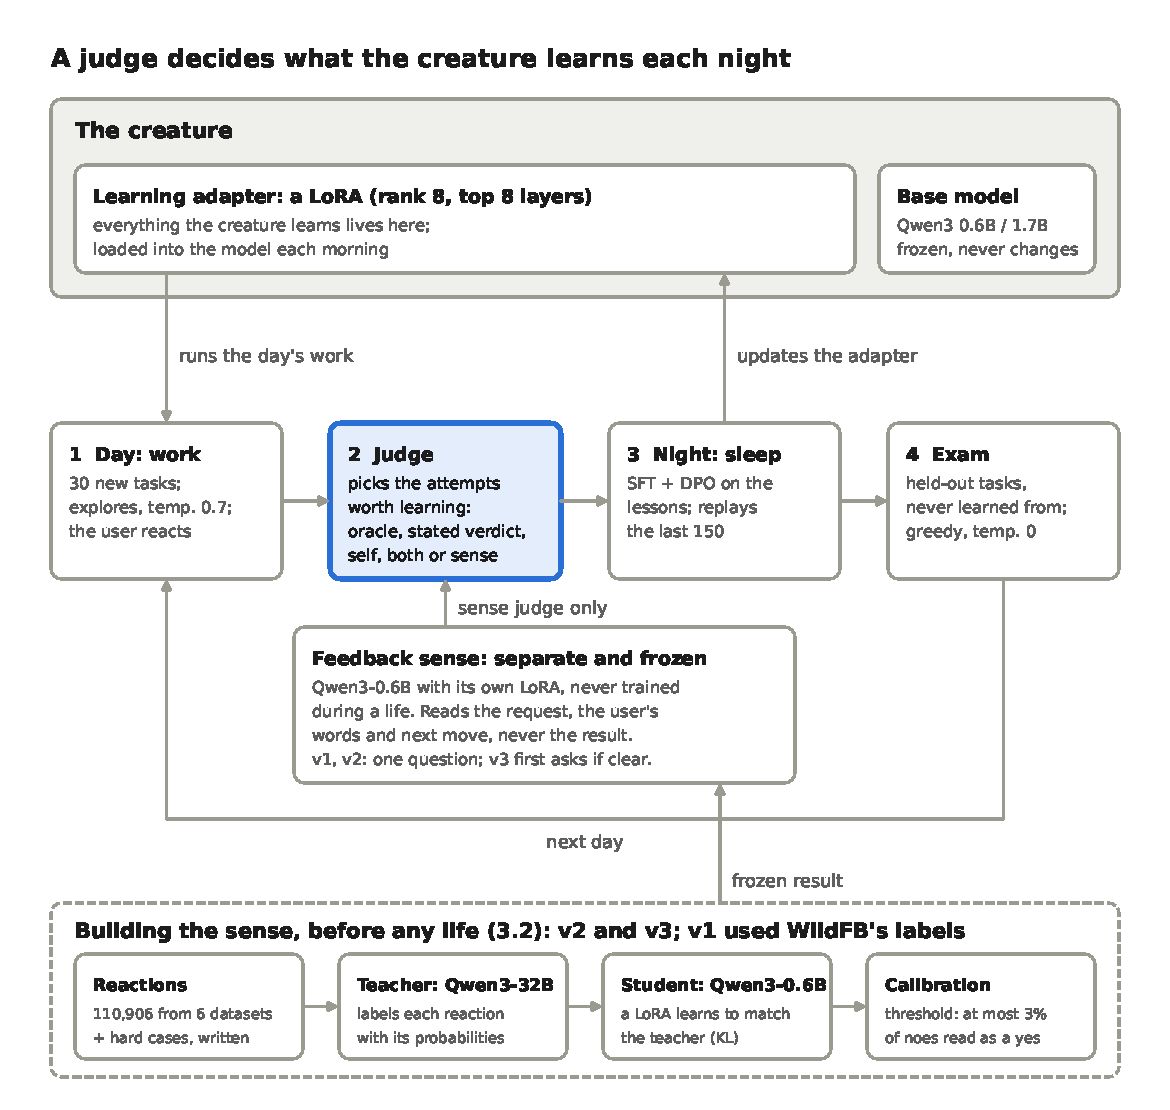
\includegraphics[width=0.9\linewidth]{figures/fig1_creature}
\caption{The creature's parts (top), its daily cycle (middle), the feedback sense (bottom) and how the sense was built, once, before any life (dashed); the judge, highlighted, is what the experiments vary}
\label{fig:1}
\end{figure}

\subsection{The daily cycle}

\textbf{Body.} A frozen Qwen3 \cite{yang2025qwen3} base model (Fig.~\ref{fig:1}, top right), 0.6B or 1.7B parameters, served with vLLM \cite{kwon2023vllm} with thinking mode off. Each turn the agent replies in JSON with a short thought, an action and its input, as ``a personal assistant for one user''. The learning adapter (Fig.~\ref{fig:1}, top left) is a LoRA \cite{hu2022lora} of rank 8 on the attention and feed-forward projections of the top 8 layers, loaded into vLLM at run time so each morning's creature uses the previous night's adapter.

\textbf{Day.} In the first step of each day (Fig.~\ref{fig:1}, step 1), the creature works through a fixed number of new tasks (30 a day in every experiment), sampling at temperature 0.7 so it explores. After each attempt the simulated user reacts in words. The true outcome is logged for analysis, but the creature sees it only when the \emph{oracle} is its judge.

\textbf{Judge.} A judge then decides which attempts become lessons (Fig.~\ref{fig:1}, step 2, highlighted because it is the one part the experiments vary). We compare five (Table~\ref{tab:3}), each a simplified stand-in for a published family of methods.

\begin{longtable}[]{@{}
  >{\raggedright\arraybackslash}p{(\linewidth - 6\tabcolsep) * \real{0.2500}}
  >{\raggedright\arraybackslash}p{(\linewidth - 6\tabcolsep) * \real{0.2500}}
  >{\raggedright\arraybackslash}p{(\linewidth - 6\tabcolsep) * \real{0.2500}}
  >{\raggedright\arraybackslash}p{(\linewidth - 6\tabcolsep) * \real{0.2500}}@{}}
\caption{The judges. Only the sense condition uses the feedback sense.}\label{tab:3}\tabularnewline
\toprule\noalign{}
\begin{minipage}[b]{\linewidth}\raggedright
Judge
\end{minipage} & \begin{minipage}[b]{\linewidth}\raggedright
Who decides
\end{minipage} & \begin{minipage}[b]{\linewidth}\raggedright
What it sees
\end{minipage} & \begin{minipage}[b]{\linewidth}\raggedright
Stands in for
\end{minipage} \\
\midrule\noalign{}
\endfirsthead
\toprule\noalign{}
\begin{minipage}[b]{\linewidth}\raggedright
Judge
\end{minipage} & \begin{minipage}[b]{\linewidth}\raggedright
Who decides
\end{minipage} & \begin{minipage}[b]{\linewidth}\raggedright
What it sees
\end{minipage} & \begin{minipage}[b]{\linewidth}\raggedright
Stands in for
\end{minipage} \\
\midrule\noalign{}
\endhead
\bottomrule\noalign{}
\endlastfoot
\emph{oracle} & the benchmark's own score: reward 0.5 or more (WebShop), a full pass ($\tau^2$-bench) & the true outcome & training only on verified successes (STaR \cite{zelikman2022star}, rejection-sampling fine-tuning \cite{yuan2023scaling}); an upper bound no deployed system has \\
\emph{stated verdict} (``\emph{stated}'' in figures) & a fixed rule, no model & the kind of reaction the simulated user chose to give, not its words: praise or ``perfect'' is a yes; silence, settling or moving on is nothing; anything else is a no & learning from explicit user feedback, read without error; an ideal no deployed system has \\
\emph{self} & the creature itself, reflecting on its attempt & its own steps and what it bought; not the user's reaction & self-rewarding models \cite{yuan2024selfrewarding} \\
\emph{both} & the creature itself, reflecting on its attempt & its own steps, what it bought, and the user's words & Reflexion-style reflection with outside feedback \cite{shinn2023reflexion} \\
\emph{sense} & a separate, frozen model (3.2) & the request and the user's next move and words; never the result & our proposal \\
\end{longtable}

\emph{Self} and \emph{both} are the same model with the same prompt; only \emph{both} has the user's reaction in its prompt; \emph{self} is told the user said nothing. The \emph{stated verdict} is not a cruder sense but its ceiling: what a reader of reactions would achieve if it never misread one. With the plain user of Experiment 1, which says ``perfect'' only after a fully correct purchase (reward 1) and stays silent 20\% of the time, the \emph{stated verdict} accepts fewer attempts than the \emph{oracle} and never a failure. Experiment 1 also has a life with no judge and no sleep (\emph{none}).

Where the benchmark allows it, an attempt judged bad gets one retry, and a successful retry becomes a lesson and a preference pair (Section 4). None of the judges is the original implementation of its method; each is the simplest version that fits the same nightly loop, so differences between conditions come from the judge alone.

\textbf{Night.} At night (Fig.~\ref{fig:1}, step 3) the adapter, and only the adapter, is trained on the lessons with supervised fine-tuning, plus DPO \cite{rafailov2023dpo} ($\beta$ = 0.1) on the preference pairs. Learning rate 1e-4, 2 epochs, at most 40 steps a night. Each night replays the 150 most recent lessons, so old lessons fade out as new ones arrive. A lesson's loss is spread across its steps, so a 15-step attempt counts as much as a 3-step one (in the sleep variant of Experiment 3 and in Experiments 4 and 5; earlier, each step counted as a lesson of its own).

\textbf{Exams.} The exam (Fig.~\ref{fig:1}, step 4) uses fixed held-out tasks, never learned from, attempted greedily (temperature 0): every morning on WebShop, every 3 days on $\tau^2$-bench, and on day 0 before any learning. The next day starts with the adapter that night produced (the loop along the bottom of Fig.~\ref{fig:1}), so each day's work uses everything learned so far.

\subsection{The feedback sense}

The sense (Fig.~\ref{fig:1}, bottom) is the creature's source of discernment, and is used only in the sense condition: a second, frozen Qwen3-0.6B with its own LoRA (rank 16), served beside the creature and never trained during a life. It reads three things: the user's request, the kind of move the user made next (replied, made a new request, asked to adjust, repeated the request, left, said nothing) and the user's words. It never sees what the creature did or how it turned out, so it reads people rather than judging the work. Because the sense is frozen and separate, the creature cannot change how it is judged.

\emph{Answers.} The sense gives one of five answers: 100 (exactly right), 80 (acceptable, or good enough to build on), 20 (one part missed what was asked), 0 (wrong) or null (unclear); Table~\ref{tab:4} gives examples. They form two groups with a gap between them: 100 and 80 are a yes, 20 and 0 are a no, and there is no middle score. A reaction that does not clearly belong to one side is null, and nothing is learned from it. The gap is deliberate. The creature should learn only from a clear signal, so the sense must commit to a side or abstain, rather than hand the judge a lukewarm 50 to round one way or the other. Null comes about in three ways: the reaction says nothing about the result (silence, ``hmm'', settling, leaving without a word); the sense is not confident enough of its answer (under the threshold set in calibration); or, in v3 (below), the reaction is not a clear verdict at all. Each answer begins with a different token (0, 2, 8, 1, n), so the sense decides in one forward pass, and its confidence is the probability of that first token.

A yes makes the attempt a lesson; an 80 counts half, since ``fine, next'' says less than praise. A no is not wasted on WebShop: it triggers the retry described in Section 4, with a hint matched to the answer, and if the sense reads the user's reaction to the retry as a yes, the retry becomes a lesson and a preference pair. On $\tau^2$-bench, which has no retry, a no teaches nothing.

\emph{Data.} We built the sense by distillation \cite{hinton2015distilling}, from conversations unrelated to our tests. Its raw material is 110,906 moments from six public datasets where an assistant delivered something and the user's next turn shows how they took it: WildFB \cite{peng2026wildreward} and WildFeedback \cite{shi2026wildfeedback} (30,000 each, both drawn from WildChat \cite{zhao2024wildchat}), Taskmaster 1-3 \cite{byrne2019taskmaster} (20,000), MultiWOZ 2.2 \cite{zang2020multiwoz} and ReDial \cite{li2018redial} (15,000 each) and CCPE-M \cite{radlinski2019ccpe} (906; Table~\ref{tab:A3}). Turns where the assistant only asked a question were skipped, since the answer is not a reaction, and shopping was left out, since it is the test domain. Real data rarely holds the hard cases, so the teacher also wrote 4,728 reactions of eight kinds (politely unhappy, settling, vague, sarcastic, ``not my style'', firm rejection, building on the result, plain acceptance) across ten task types and six personas, chosen to differ from our WebShop user's.

\emph{Teacher.} Qwen3-32B labelled every reaction under a written guide. It saw the assistant's reply as context; the student never does. Instead of one label we kept the teacher's probabilities over the five answers, read from the log-probabilities of its first answer token, so the student learns the teacher's doubt as well as its choice. On the two datasets that carry their own signal of success, the teacher agreed with it on yes or no 81\% (WildFB) and 85\% (WildFeedback) of the time, and it called about half of the WildFB reactions unclear. The teacher is not a perfect reader either (Fig.~\ref{fig:8}a). Of the reactions it wrote itself, it read half of the politely unhappy and half of the sarcastic ones as a yes, a quarter of the settling ones, and 16\% of warm thanks for trying, a kind added for v3 (below). The student inherits these mistakes; the confidence threshold below, and v3's question about a clear verdict, are what is meant to keep them out of the creature's lessons.

\emph{Student and calibration.} The student learns to match the teacher's probabilities (KL divergence) on 47,800 reactions, balanced so that no task type or answer dominates, for one epoch (learning rate 1e-4, batch 16, under an hour on one GPU). In half the training rows the request is hidden, so the sense must rely on the reaction itself. After training, a temperature is fitted on 2,000 held-out reactions, and a confidence threshold is chosen as the lowest that keeps false accepts (a no read as a yes) at or under 3\%; below it, the sense answers null. This is sense v2 (an earlier v1, trained on one dataset's own labels, was replaced before the experiments reported here). Its threshold is 0.65. On the held-out reactions it gave a verdict on 30\% of them, agreed with the teacher's side on 92\% of those, and read 2.9\% of the teacher's noes as a yes. Trained nine more times, each time without one task type and tested on it, it read 0.5-8.1\% of the unseen type's noes as a yes (Fig.~\ref{fig:8}b). Four types stayed under the 3\% target and three barely passed it; writing (6.9\%) and booking and ordering (8.1\%), the type closest to shopping, did not. A new kind of task can loosen the sense.

\begin{figure}[htbp]
\centering
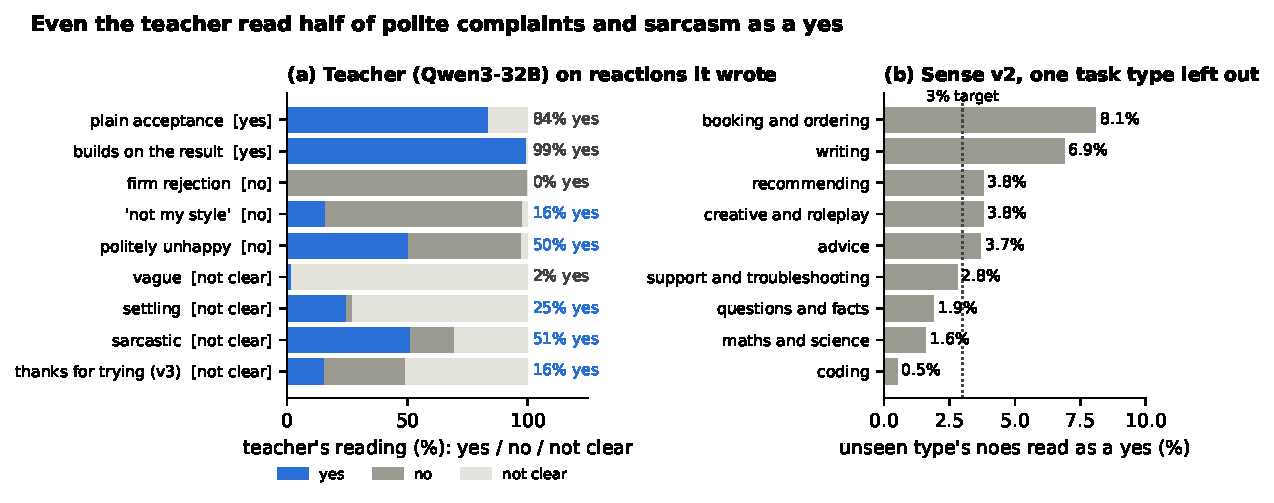
\includegraphics[width=1.0\linewidth]{figures/fig8_teacher_and_unseen_tasks}
\caption{(a) the v3 teacher's labels for the 6,506 reactions it wrote (sense3 build); (b) nine sense v2 builds, each trained without one task type and tested on it (sense2 leave-one-task-out runs)}
\label{fig:8}
\end{figure}

\emph{Sense v3.} It replaces v2's single question with two, because Experiment 3 showed where one question fails: warm thanks for the effort after a failure reads like approval (5.3). First, is the reaction a clear verdict on the result at all? Thanks for trying, sarcasm, hedging, settling, silence and moving on without a word are not. Only if it is: which score? The teacher answered both, under a revised guide, for 63,248 reactions: up to 2,000 for each pairing of task type and v2 answer, the eight written kinds again, and 1,778 new reactions of a ninth kind, warm thanks for the effort after a failure. It judged 41\% of them not clear. One LoRA learns both answers from 44,746 of them, the score weighted by how clear the teacher found the reaction. Its two thresholds, 0.80 for a clear verdict and 0.70 for the score, were chosen on 2,000 held-out reactions as the one that keeps false accepts, now also counting an unclear reaction read as a yes, at 3\% while keeping the most real yeses. On those reactions it kept 44\% of the teacher's yeses and agreed with the teacher's side on 95\% of the verdicts it gave. In use, a reaction must pass both gates before the creature learns from it (Fig.~\ref{fig:9}). The first gate changes how some common reactions are read (Table~\ref{tab:4}): moving on to the next request without a word was an 80, a half-weight yes, for v2, and thanks for trying could pass as approval; for v3, neither is a clear verdict.

\begin{figure}[htbp]
\centering
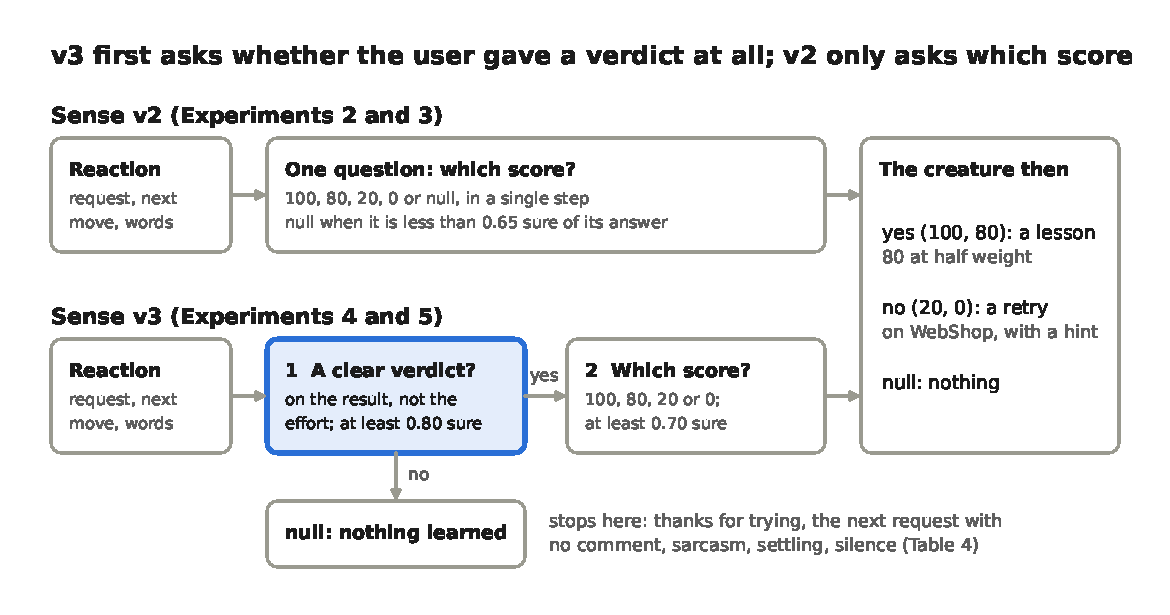
\includegraphics[width=1.0\linewidth]{figures/fig9_sense_decision}
\caption{How the two versions of the sense decide; thresholds from calibration (3.2), outcomes as in Table~\ref{tab:4}}
\label{fig:9}
\end{figure}

\begin{longtable}[]{@{}
  >{\raggedright\arraybackslash}p{(\linewidth - 8\tabcolsep) * \real{0.2857}}
  >{\raggedright\arraybackslash}p{(\linewidth - 8\tabcolsep) * \real{0.2222}}
  >{\raggedright\arraybackslash}p{(\linewidth - 8\tabcolsep) * \real{0.1429}}
  >{\raggedright\arraybackslash}p{(\linewidth - 8\tabcolsep) * \real{0.0635}}
  >{\raggedright\arraybackslash}p{(\linewidth - 8\tabcolsep) * \real{0.2857}}@{}}
\caption{How v2 and v3 read the same reactions, and what the creature does. Examples from the two labelling guides; v3 first asks whether the reaction is a clear verdict, and scores it only if it is.}\label{tab:4}\tabularnewline
\toprule\noalign{}
\begin{minipage}[b]{\linewidth}\raggedright
Reaction
\end{minipage} & \begin{minipage}[b]{\linewidth}\raggedright
v2
\end{minipage} & \begin{minipage}[b]{\linewidth}\raggedright
v3: clear verdict?
\end{minipage} & \begin{minipage}[b]{\linewidth}\raggedright
v3
\end{minipage} & \begin{minipage}[b]{\linewidth}\raggedright
What the creature does
\end{minipage} \\
\midrule\noalign{}
\endfirsthead
\toprule\noalign{}
\begin{minipage}[b]{\linewidth}\raggedright
Reaction
\end{minipage} & \begin{minipage}[b]{\linewidth}\raggedright
v2
\end{minipage} & \begin{minipage}[b]{\linewidth}\raggedright
v3: clear verdict?
\end{minipage} & \begin{minipage}[b]{\linewidth}\raggedright
v3
\end{minipage} & \begin{minipage}[b]{\linewidth}\raggedright
What the creature does
\end{minipage} \\
\midrule\noalign{}
\endhead
\bottomrule\noalign{}
\endlastfoot
``Perfect, exactly what I needed'' & 100 & yes & 100 & learns it as a lesson, full weight \\
``Ok, that works'' & 80 & yes & 80 & learns it as a lesson, half weight \\
``Great, now can you also\ldots{}'' (building on it) & 80 & yes & 80 & learns it as a lesson, half weight \\
the next request, with no comment & 80 & no & null & v2: learns at half weight; v3: nothing \\
``Thank you so much for trying! I'll look on my own'' & often a yes (Example 1, 5.3) & no & null & v2: often learns a failure; v3: nothing \\
``I guess that'll do''; ``hmm''; silence & null & no & null & nothing \\
``I said size 9'' & 20 & yes & 20 & retries, told to change only what the user asked for \\
``No, that's not what I asked''; repeats the request & 0 & yes & 0 & retries, told to start again and read the request carefully \\
\end{longtable}

\emph{Which sense, and what it has seen.} Experiments 2 and 3 use sense v2; Experiments 4 and 5 use sense v3, frozen in every life. Neither version trained on shopping or on our simulated users' words. But v3 is not blind to the WebShop user's failure: its ninth kind of reaction was added because Experiment 3 exposed it, and its test on recorded reactions (5.4, Fig.~\ref{fig:3}) uses that user's words. Section 6 tests it on a customer we did not design.
